\documentclass{beamer}

\usetheme{Boadilla}

%\includeonlyframes{current}

\usepackage{times}
\usefonttheme{structurebold}
\usepackage{listings}

\usepackage{pgf}
\usepackage{tikz}
\usepackage{alltt}
\usepackage[normalem]{ulem}
\usetikzlibrary{arrows}
\usetikzlibrary{automata}
\usetikzlibrary{shapes}
\usepackage{amsmath,amssymb}
\usepackage{rotating}
\usepackage{ulem}
\usepackage{listings}
\usepackage{enumerate}

%\setbeamercovered{dynamic}
\setbeamertemplate{footline}[page number]{}
\setbeamertemplate{navigation symbols}{}
\usefonttheme{structurebold}

\title{SE 101---Lecture 10}
\author{Patrick Lam\\University of Waterloo}
\date{November 15, 2016}

\colorlet{redshaded}{red!25!bg}
\colorlet{shaded}{black!25!bg}
\colorlet{shadedshaded}{black!10!bg}
\colorlet{blackshaded}{black!40!bg}

\colorlet{darkred}{red!80!black}
\colorlet{darkblue}{blue!80!black}
\colorlet{darkgreen}{green!80!black}

\newcommand{\rot}[1]{\rotatebox{90}{\mbox{#1}}}
\newcommand{\gray}[1]{\mbox{#1}}

\newenvironment{changemargin}[1]{% 
  \begin{list}{}{% 
    \setlength{\topsep}{0pt}% 
    \setlength{\leftmargin}{#1}% 
    \setlength{\rightmargin}{1em}
    \setlength{\listparindent}{\parindent}% 
    \setlength{\itemindent}{\parindent}% 
    \setlength{\parsep}{\parskip}% 
  }% 
  \item[]}{\end{list}}


\lstset{ %
language=Java,
basicstyle=\ttfamily,commentstyle=\scriptsize\itshape,showstringspaces=false,breaklines=true}

\begin{document}

\begin{frame}
  \titlepage
\end{frame}

\begin{frame}
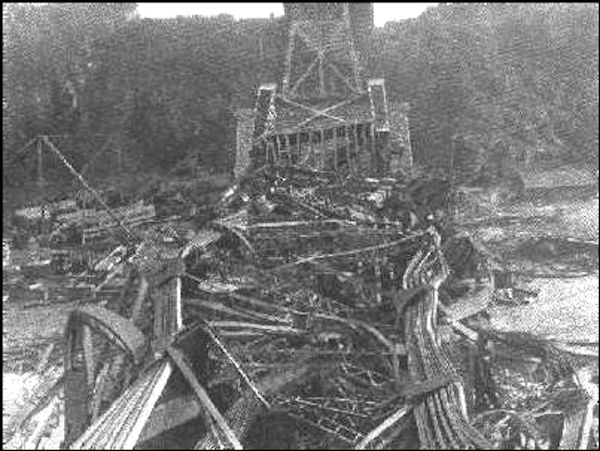
\includegraphics[width=\textwidth]{images/Quebec_Bridge_Collapse_of_1907.jpg}
\end{frame}

\begin{frame}
\begin{center}
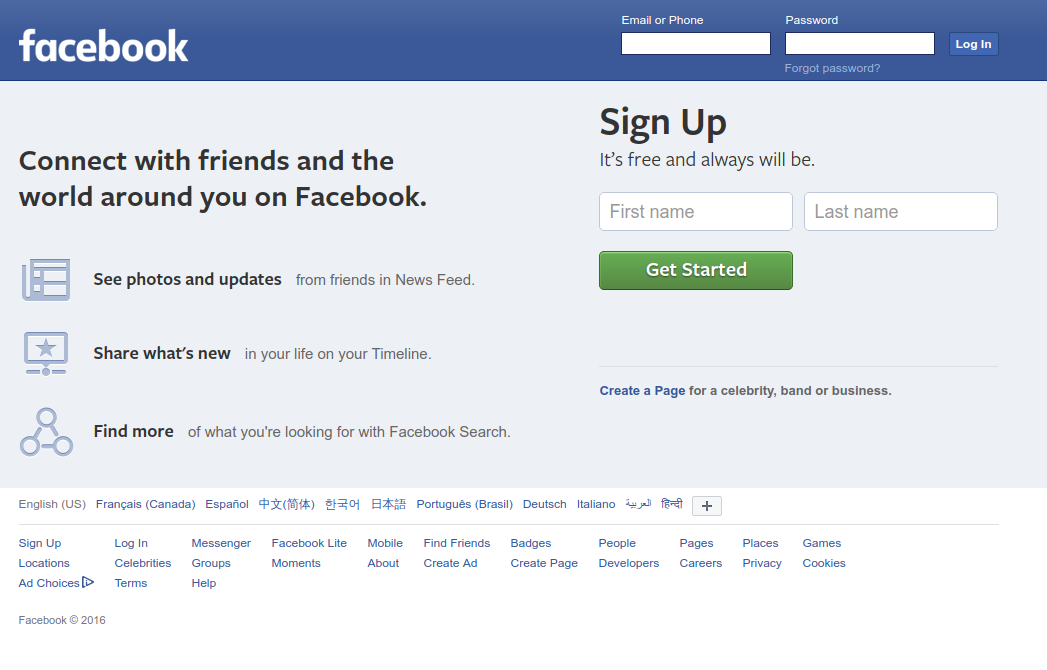
\includegraphics[width=\textwidth]{images/fb.png}
\end{center}
\end{frame}

\begin{frame}
\frametitle{Questions}
\begin{itemize}
\item What is FB's primary goal?
\item How does it make money?
\item How does it make more money?
\end{itemize}
\end{frame}

\begin{frame}
\frametitle{More Questions: Behaviour}
\begin{itemize}
\item How can Facebook affect behaviour?
\item How do we know that Facebook affects behaviour?
\end{itemize}
\end{frame}

\begin{frame}
\frametitle{News Feed}
Propose a change to the newsfeed algorithm.
\begin{itemize}
\item What are the economic, social and technological implications?
\end{itemize}
\end{frame}

\begin{frame}
\begin{center}
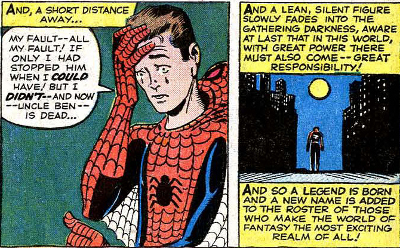
\includegraphics{images/spider400.jpg}
\end{center}
\end{frame}

\begin{frame}
\frametitle{Responsibility}

\begin{itemize}
\item Describe one direct, concrete harm to a specific person that Facebook has facilitated.
\item Suggest a way that Facebook could mitigate the harm.
\end{itemize}
\end{frame}

\end{document}
